\tikzset{%
    every neuron/.style={
        circle,
        draw,
        minimum size=5pt,
        inner sep=0pt,
        very thin
    },
    neuron/.style={
        fill
    },
}

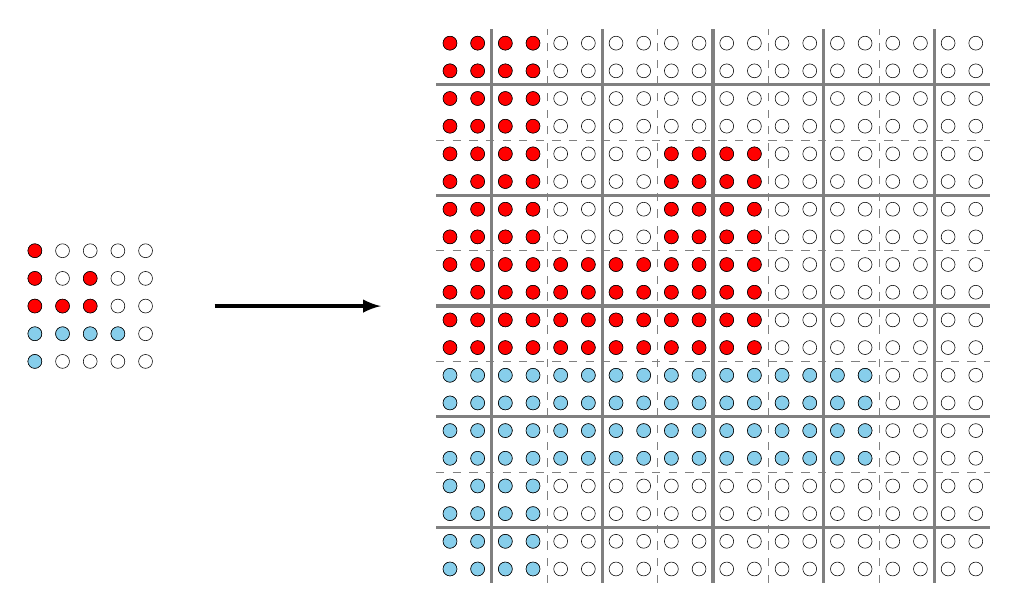
\begin{tikzpicture}[x=0.8cm, y=0.8cm, >=latex, every text node part/.style={align=center}]

    %% BEGIN small grid
    \foreach \x in {0,...,4}
        \foreach \y in {0,...,4} {
            \pgfmathtruncatemacro{\label}{\x*102+\y}
            \node [every neuron/.try] (\label) at (10pt*\x-150pt,10pt*\y+75pt) {};
        } 
    % \foreach \x in {0,...,4}
    %     \foreach \y in {0,...,3} {
    %         \pgfmathtruncatemacro{\label}{\x*102+\y}
    %         \pgfmathtruncatemacro{\labell}{\x*102+\y+1}
    %         \path[very thin] (\label) edge (\labell);
    %     }
    % \foreach \x in {0,...,3}
    %     \foreach \y in {0,...,4} {
    %         \pgfmathtruncatemacro{\label}{\x*102+\y}
    %         \pgfmathtruncatemacro{\labell}{\x*102+\y+102}
    %         \path[very thin] (\label) edge (\labell);
    %     }
    \foreach \x/\y in {0/0, 0/1, 1/1, 2/1, 3/1} {
        \node [every neuron/.try, fill=SkyBlue] () at (10pt*\x-150pt,10pt*\y+75pt) {};
    }
    \foreach \x/\y in {0/4, 0/3, 0/2, 1/2, 2/2, 2/3} {
        \node [every neuron/.try, fill=Red] () at (10pt*\x-150pt,10pt*\y+75pt) {};
    }
    %% END small grid

    %% BEGIN large grid
    \foreach \x in {0,...,19}
        \foreach \y in {0,...,19} {
            \pgfmathtruncatemacro{\label}{\x*102+\y+3456}
            \node [every neuron/.try] (\label) at (10pt*\x,10pt*\y) {};
        } 
    \foreach \x in {1,...,4} {
        \path[very thin, gray, dashed] (40pt*\x-5pt, -5pt) edge (40pt*\x-5pt, 195pt);
    }
    \foreach \x in {0,...,4} {
        \path[very thick, gray] (40pt*\x+15pt, -5pt) edge (40pt*\x+15pt, 195pt);
    }
    \foreach \x in {1,...,4} {
        \path[very thin, gray, dashed] (-5pt, 40pt*\x-5pt) edge (195pt, 40pt*\x-5pt);
    }
    \foreach \x in {0,...,4} {
        \path[very thick, gray] (-5pt, 40pt*\x+15pt) edge (195pt, 40pt*\x+15pt);
    }
    \foreach \x/\y in {0/0, 0/1, 1/1, 2/1, 3/1} 
        \foreach \a in {0,...,3}
            \foreach \b in {0,...,3} {
                \node [every neuron/.try, fill=SkyBlue] () at (40pt*\x + 10pt*\a,40pt*\y + 10pt*\b) {};
            }
    
    \foreach \x/\y in {0/4, 0/3, 0/2, 1/2, 2/2, 2/3} 
        \foreach \a in {0,...,3}
            \foreach \b in {0,...,3} {
                \node [every neuron/.try, fill=Red] () at (40pt*\x + 10pt*\a,40pt*\y + 10pt*\b) {};
            }
    \path[->, very thick] (-85pt, 95pt) edge (-25pt, 95pt);
    %% END large grid
\end{tikzpicture}